\section{Hello World}

Ready for creating your first SuperCollider program? Assuming you have SC up and running in front of you, open a new document (menu File$\rightarrow$New, or shortcut [ctrl+N]) and type the following line:

 
\begin{lstlisting}[style=SuperCollider-IDE, basicstyle=\scttfamily\footnotesize ]
"Hello World".postln;
\end{lstlisting}
 

Leave your cursor anywhere in that line (it doesn't matter if beginning, middle, or end). Press [ctrl+Enter] to evaluate the code. ``Hello world'' appears in the Post window. Congratulations! That was your first SuperCollider program.

 
\bigskip
\todo[inline, color=green!40]{ TIP: Throughout this document, ctrl (control) indicates the modifier key for keyboard shortcuts that is used on Linux and Windows platforms. On Mac OSX, use cmd (command) instead. }
\bigskip
 

Figure \ref{fig:scidegui} shows a screenshot of the SuperCollider IDE (Integrated Development Environment) when you first open it. Let's take a moment to get to know it a bit.

\begin{figure}[t]
\centerline{\framebox{
	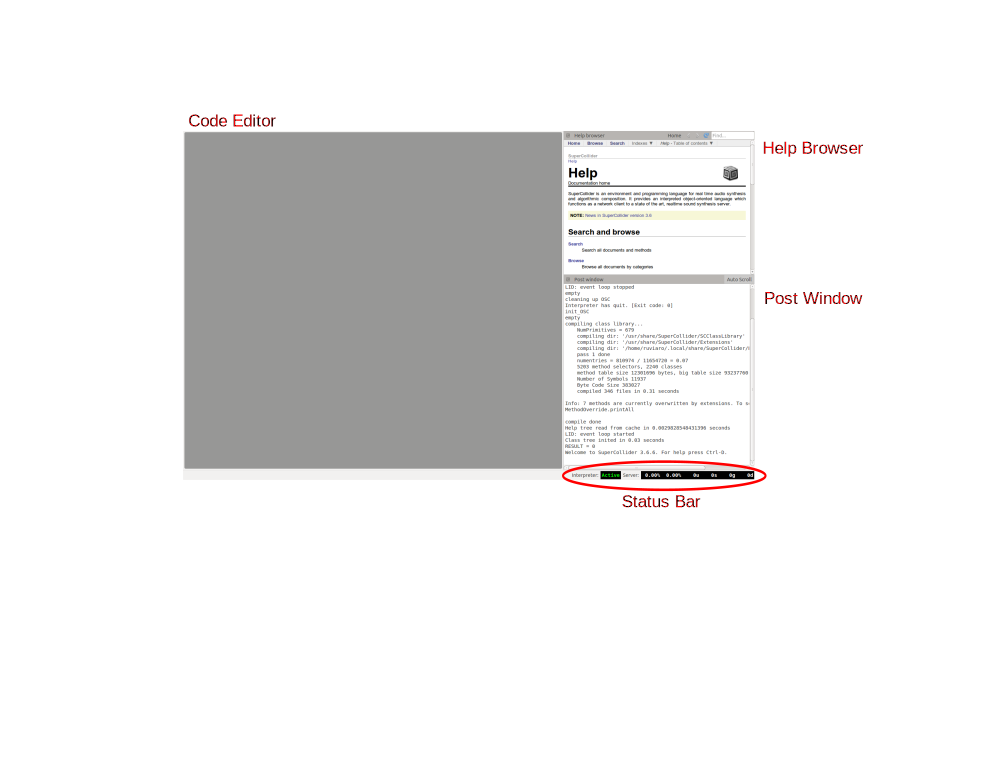
\includegraphics[width=0.7\columnwidth]{fig-supercollider-ide-2.png}}}
\caption{SuperCollider IDE interface.}
\label{fig:scidegui}
\end{figure}

What is the SuperCollider IDE? It is ``a cross-platform coding environment developed specifically for SuperCollider (\dots), easy to start using, handy to work with, and sprinkled with powerful features for experienced coders. It is also very customizable. It runs equally well and looks almost the same on Mac OSX, Linux and Windows.''\footnote{Quoted from the SuperCollider Documentation: \url{http://doc.sccode.org/Guides/SCIde.html}. Visit that page to learn more about the IDE interface.}

The main parts you see on the SC window are the Code Editor, the Help Browser, and Post Window. If you don't see any of these when you open SuperCollider, simply go to the menu View$\rightarrow$Docklets (that's where you can show or hide each of them). There is also the Status Bar, always located on the bottom right corner of the window.

Always keep the Post window visible, even if you don't understand yet all the stuff being printed there. The Post window displays the responses of the program to our commands: results of code evaluation, various notifications, warnings, errors, etc.

\bigskip
\todo[inline, color=green!40]{ TIP: You can temporarily enlarge and reduce the editor font size with the shortcuts [Ctrl++] and [Ctrl+-] (that's the control key together with the plus or minus keys, respectively). If you are on a laptop without a real plus key, use [Ctrl+shift+=].}
\bigskip


